\chapter{Technology Review}

\section{Multi-Tenant Database Architectures}
A multi-tenant system provides one shared instance of an application and its infrastructure to multiple users, referred to as tenants, while maintaining the logical separation of their data. In a SaaS context, tenants
are typically organisations or businesses that each require their own private view
of the data. How that separation is achieved at the database level is one of the
most important design decisions in a SaaS application, as it determines the
system's performance, security, operational cost, and ability to
scale \cite{wangStudyPerformanceEvaluation2008}.

\subsection*{Different Types of Multi-Tenant Database Designs}
The multi-tenant database design can be broken down into three primary isolation
models, as defined by Karat\c{a}s et al. \cite{karatasMultitenantArchitecturesCloud2017} and illustrated in Figure~\ref{fig:isolation-patterns}.

\begin{figure}[htbp]
    \centering
    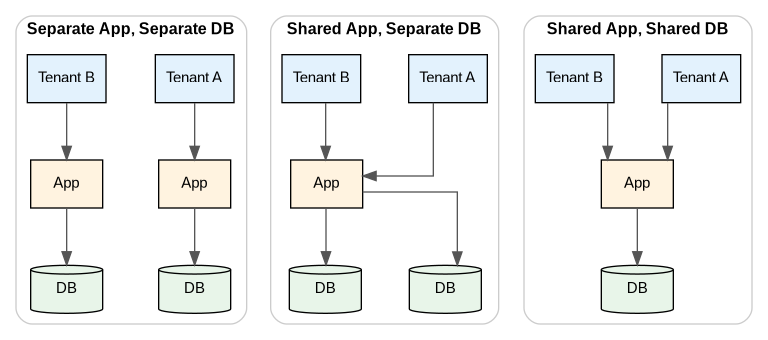
\includegraphics[width=\textwidth]{images/isolation-patterns.png}
    \caption{Multi-tenant database isolation patterns}
    \label{fig:isolation-patterns}
\end{figure}

\textbf{Separate Application, Separate Database} gives each tenant a fully
independent application instance and database. Data isolation is guaranteed: there
is no shared infrastructure at the database layer, so there is no risk of one
tenant accessing another's data. The trade-off is cost and operational overhead.
Every new tenant requires provisioning an additional stack, and hardware resources
cannot be shared across tenants, making this model expensive to operate at scale
\cite{karatasMultitenantArchitecturesCloud2017}.

\textbf{Shared Application, Separate Database} retains a single application
instance but still provides each tenant with its own database. This reduces
application-layer overhead while preserving data isolation.
It is still expensive in terms of storage and database management, since the number of databases grows linearly with the number of tenants.

\textbf{Shared Application, Shared Database} is the most resource-efficient
model. All tenants share the same application and the same database, with data
partitioned logically rather than physically. This model has two variants. In
\textit{Shared Database, Separate Schema}, each tenant receives its own set of
tables within the shared database. In \textit{Shared Database, Shared Schema},
all tenants share the same tables, and their rows are distinguished by a
\texttt{tenant\_id} column. The shared schema variant offers the highest resource
utilisation and the lowest per-tenant cost, but it places a burden on
the data isolation mechanisms, since a missing or incorrect filter predicate could
expose one tenant's data to another \cite{wangStudyPerformanceEvaluation2008}.

\subsection*{Trade-offs: Isolation vs.\ Efficiency vs.\ Cost}
The selection of an isolation model is not a decision that can optimise all
dimensions simultaneously. Wang et al.\ \cite{wangStudyPerformanceEvaluation2008} established the foundational tension: higher isolation means better security but limits the
number of tenants a system can support on fixed hardware. Zhou et al.\
\cite{zhouDB2MMTMassiveMultitenant2011} quantify this directly on IBM DB2, demonstrating that a shared table model (S3) supports approximately 400 concurrent tenants on the same
hardware that a separate database model (S1) can sustain only around 8. The
capacity advantage of the shared approach is significant, but it depends
on effective isolation being built into the system.

Cost is yet another concern. Wang et al.\ \cite{wangStudyPerformanceEvaluation2008} categorise multi-tenant system costs across three dimensions: infrastructure
(hardware, software, and utilisation), management (lifecycle, monitoring, and
backup), and development (tenant-specific customisation). Shared architectures
reduce infrastructure and management costs substantially. Aulbach et al.\
\cite{aulbachExtensibilityDataSharing2011} and Yaish and Goyal \cite{yaishMultitenantDatabaseArchitecture2013} both demonstrate that
shared schemas lower Total Cost of Ownership by eliminating per-tenant schema
provisioning and by enabling self-service configuration. However, neither work
quantifies how the cost of securing a shared schema compares to the cost of
stronger physical isolation.

Performance also needs to be taken into account. Wang et al.\ \cite{wangStudyPerformanceEvaluation2008}
measured that adding Label-Based Access Control (LBAC) - a database-level
security mechanism - reduced throughput by 15\% compared to less secure approaches.
Ni et al.\ \cite{niAdaptiveDatabaseSchema2014} propose the ADAPT methodology, which improves query performance by 2--3$\times$ over static shared-schema approaches by dynamically
clustering attributes based on workload, but their evaluation explicitly assumes
application-level filtering and tests no security mechanisms. The pattern is
consistent across the literature: studies that optimise performance assume the
security problem is solved elsewhere, and studies that address security do not
measure the performance impact of their mechanisms \cite{karatasMultitenantArchitecturesCloud2017, battulaSystematicReviewMultitenant2024}.

\subsection*{Data Isolation Techniques}
Within the shared database, shared schema model, the mechanisms used to enforce
tenant data isolation fall into two categories: filter-based and
permission-based.

Filter-based isolation is implemented at the application layer by appending a
tenant identifier predicate to every query, typically expressed as
\texttt{WHERE tenant\_id = ?}. Wang et al.\ \cite{wangStudyPerformanceEvaluation2008} identify this as the
most common approach in practice due to its simplicity. Its critical weakness is
that isolation is only as reliable as the application code: a missing predicate,
a buggy query, or a SQL injection vulnerability can expose data across tenant
boundaries. Gupta, Kumar, and Agnihotri \cite{guptaDataIsolationMultitenant2016} extend this approach with session-based identifiers that rotate periodically, reducing injection risk, but their mechanism remains dependent on the application being free of errors.

Permission-based isolation enforces tenant boundaries at the database engine
level, independently of the application. PostgreSQL Row-Level Security is
a prominent example: policies are attached directly to tables, and the database
engine automatically appends the isolation predicate to every qualifying query
before execution, regardless of what the application sends. Factor et al.\
\cite{factorSecureLogicalIsolation2013} formalise the principles underpinning this approach in their SLIM (Secure Logical Isolation for Multi-tenancy) model, based on least privilege, tenant containment, escalation avoidance, and minimising attack surface. The advantage of database-level isolation is that it acts as a safety net: even if the application layer has a bug, the database will not return rows belonging to another tenant. The documented trade-off is a performance overhead from the additional policy evaluation on every query.

\section{Related Works}
This section examines specific studies that have proposed techniques for managing multi-tenant data and prior systematic reviews that establish the broader research context.

\subsection*{Proposed Multi-Tenant SaaS Database Design Patterns}
Several studies have proposed specific techniques for managing multi-tenant data
that are directly relevant to the design decisions made in this project.

Ni et al.\ \cite{niAdaptiveDatabaseSchema2014} introduce \textbf{ADAPT} (Adaptive Database Schema Design for
Multi-Tenant Data Management), a methodology that dynamically reorganises table
schemas by clustering attributes based on observed query workloads. ADAPT achieves
a 2--3$\times$ throughput improvement over static shared-schema designs and
demonstrates reasonable scalability up to 4,000 tenants, at which point the
alternative individual-table approach degrades severely. Its limitation for this
project's context is that it assumes application-level filtering and does not
evaluate how it would work with database-level security policies.

Mangwani and Tokekar \cite{mangwaniContainerBasedScalability2022} evaluate microservice architectures as a
scalability mechanism for multi-tenant SaaS systems. Their findings show that at
low concurrency (around 50 users), monolithic and microservice architectures
perform similarly, but at high load (300+ users), microservices offer lower
response times, higher throughput, and approximately 11\% better CPU utilisation.
This supports the case for modular application design but treats the database as
a black box, with no evaluation of how schema design choices interact with
service decomposition.

Sharma and Kaur \cite{sharmaImplementingMultitenantSystem2021} demonstrate MongoDB sharding as an alternative
to relational multi-tenant designs, enabling horizontal scaling through data
partitioning across nodes with automatic load balancing. While this illustrates
the growing relevance of NoSQL approaches, the study does not compare its
performance or isolation guarantees against optimised relational alternatives,
leaving the trade-off between schema flexibility and data isolation unknown.

\subsection*{Literature Reviews}
Two prior systematic reviews are most directly relevant to this work and
establish the context into which this project's design decisions fit.

Karat\c{a}s et al.\ \cite{karatasMultitenantArchitecturesCloud2017} conducted a broad systematic mapping study
covering 407 papers from 2000 to 2017. Their key quantitative finding is that
65\% of papers preferred a shared database strategy, and 58\% were ideological
proposals without implementation. The study is descriptive rather than evaluative:
it reports which strategies are preferred but does not analyse why or evaluate
combined approaches. Its 2017 cutoff also means it predates significant
developments in containerised deployment and modern database security tooling.

Battula \cite{battulaSystematicReviewMultitenant2024} provides a more recent (2024) systematic review focused
specifically on security mechanisms in multi-tenant cloud databases, analysing 25
papers from 2012 to 2024. It comprehensively covers encryption, access control,
and threat detection, but treats performance and scalability as secondary concerns.
Like Karat\c{a}s et al., it evaluates mechanisms in isolation and identifies no
integrated approaches combining database-level security with performance
optimisation techniques.

The gap identified by both reviews, and confirmed by the broader set of papers
analysed, is the absence of empirical evaluation of combined approaches. No study
evaluates how a database-level security mechanism such as RLS performs when applied
alongside a shared schema optimised for multi-tenant query patterns, nor how much
of the performance benefit claimed by approaches like ADAPT survives the addition
of policy-based isolation. Zhu et al.\ \cite{zhuMTRPHighPerformanceCostEfficient2024} highlight an additional
dimension of this problem: optimising database performance for one tenant can
degrade it for others, a conflict that existing research leaves unresolved.

This project addresses a subset of this integration gap directly. TRiM adopts a
Shared Application, Shared Database, Shared Schema design, the pattern associated
with the highest resource efficiency, and enforces tenant isolation using
PostgreSQL Row-Level Security rather than application-layer filtering alone.
The load testing results presented in Chapter~\ref{chap:evaluation} provide
empirical evidence on the performance overhead of this combination under
real data volumes, contributing practical findings to the field.